\section{Background}\label{Sect:background}
\subsection{Linear Algebra}\label{Sect:linearAlgebra}
In order to understand how to build the models we want, we must first have a knowledge of linear algebra, data analysis, and signal processing. Imagine you are presented with the data points in Figure \ref{figFunc1Samples} as samples from a secret function. Building a function that matches the data will now be investigated.

\begin{figure}[h]
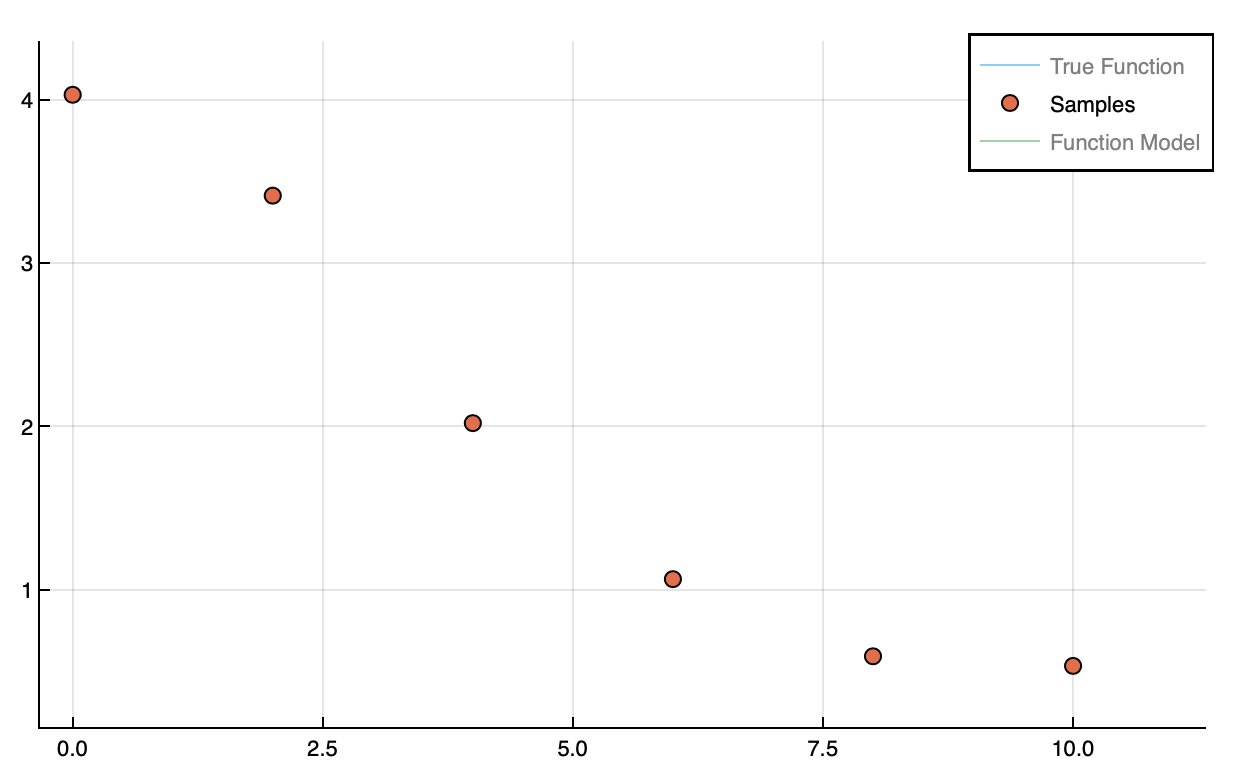
\includegraphics[scale = 0.4]{Figures/func1Samples}
\caption{An unknown function sampled by 6 data points.
\label{figFunc1Samples}} 
\end{figure}

\par Let us first make a guess of the form of the secret function. Because it looks like a simple polynomial, let us work with a power series of the form

\begin{align}
f(x) &= \sum_{n=0}^\infty b_n x^n
	\label{powerSum}\\ 
&= x^0b_0 + x^1b_1 + x^2b_2 + \ldots\ .
	\label{powerSeries}
\end{align}

\par The coefficients, $b_n$, will determine the shape of the polynomial.

Equation \ref{powerSeries} can be evaluated at $x=2$ and written in matrix form as

\begin{equation} \label{powerVectors}
\begin{bmatrix}
1 & 2 & 4 & 8 & 16
\end{bmatrix}
\begin{bmatrix}
b_0 \\
b_1 \\
b_2 \\
b_3 \\
b_4 
\end{bmatrix}
=
\begin{bmatrix}
f(2)
\end{bmatrix} .
\end{equation}

\par Equation \ref{powerVectors} is the expanded form of the fundamental linear algebra equation, 

\begin{equation} \label{fundLinAlg}
A\vec{b} = \vec{y},
\end{equation}
where $A$ is a matrix.

\par Evaluating Equation \ref{powerSeries} at all of the data points in Figure \ref{figFunc1Samples} would increase the number of rows in the matrix. Each row in the $A$ matrix corresponds to a unique sample point.

%\par Clearly with equation (\ref{powerVectors}) we can only input one point, $(x_i,f(x_i))$, which does not provide enough information to solve for reasonable values in $\vec{b}$, the vector of coefficients. In figure \ref{figFunc1Samples} we have 6 samples, so we can repeat equation (\ref{powerVectors}) for each sample with the same coefficients. We can combine all six equations into one like so

%\par Now we can see that each row in the $x$ matrix corresponds with a row in the $f(x)$ vector. Each row represents one of our sample points, thus denoting 6 rows. This relationship between rows and individual sample points can be better visualized if subscripts are added to each respective value of $x$,

\begin{equation} \label{LinAlgSubscript}
\begin{bmatrix}
1 & x_1 & x_1^2 & x_1^3 & x_1^4 \\
1 & x_2 & x_2^2 & x_2^3 & x_2^4 \\
1 & x_3 & x_3^2 & x_3^3 & x_3^4 \\
 & & \vdots & &
\end{bmatrix}
\begin{bmatrix}
b_0 \\
b_1 \\
b_2 \\
b_3 \\
b_4 
\end{bmatrix}
=
\begin{bmatrix}
f(x_1) \\ 
f(x_2) \\
f(x_3) \\ 
\vdots
\end{bmatrix}.
\end{equation}
And finally, $A$ and $\vec{y}$ can be populated with their true values,

\begin{equation} \label{realValues}
\begin{bmatrix}
1 & 0 & 0^2 & 0^3 & 0^4 \\
1 & 2 & 2^2 & 2^3 & 2^4 \\
1 & 4 & 4^2 & 4^3 & 4^4 \\
1 & 6 & 6^2 & 6^3 & 6^4 \\
1 & 8 & 8^2 & 8^3 & 8^4 \\
1 & 10 & 10^2 & 10^3 & 10^4
\end{bmatrix}
\begin{bmatrix}
b_0 \\
b_1 \\
b_2 \\
b_3 \\
b_4 
\end{bmatrix}
=
\begin{bmatrix}
f(0) \\ 
f(2) \\
f(4) \\ 
f(6) \\
f(8) \\
f(10)
\end{bmatrix}
\end{equation}

\par If the $A$ matrix were square and invertible, solving for $\vec{b}$ would be as simple as $\vec{b} = A^{-1}\vec{y}$. Because there are more equations than unknowns, this is an \textit{over-determined} system; the alternative being an \textit{under-determined} system, one with more unknowns than equations.
\par There will be either no solutions, or an infinite number of solutions. In the case of infinite solutions, the solution needs to be constrained. If there are no solutions, as is often the case with an underdetermined system, a least-squares approximation can be calculated. In either case, the solutions to the linear systems become non-unique. This means there is not a single set of values for $\vec{b}$ that can solve Equation \ref{fundLinAlg}.
\par In the example given, calculating one sample is quite easy, but in modeling more complicated systems, each sample becomes computationaly expensive. It will later be seen that the systems used will generally be underdetermined.
\par Solving an overdetermined system for the vector of coefficients can be done by 

\begin{align}
A\vec{b} &= \vec{y} \\
(A^TA)\vec{b} &= A^T\vec{y} \\
\vec{b} &= A^T\vec{y},
\end{align}
where $A^T$ denotes the transpose of $A$.

\par Solving an underdetermined system is done by SVD,

\begin{align}
A\vec{b} &= \vec{y} \\
(A^TA)\vec{b} &= A^T\vec{y} \\
\vec{b} &= A^T\vec{y}.
\end{align}

\par Now that $\vec{b}$, the vector of coefficients, has been solved for, the model can be used to predict the y position of any x value within the range of sample points. To produce a continuous visual of the model's fit, the model can take in x values for every point in the sample range and plot its respective evaluation. The result of this process can be seen in Figure \ref{figFunc1True}.

\begin{figure}[h]
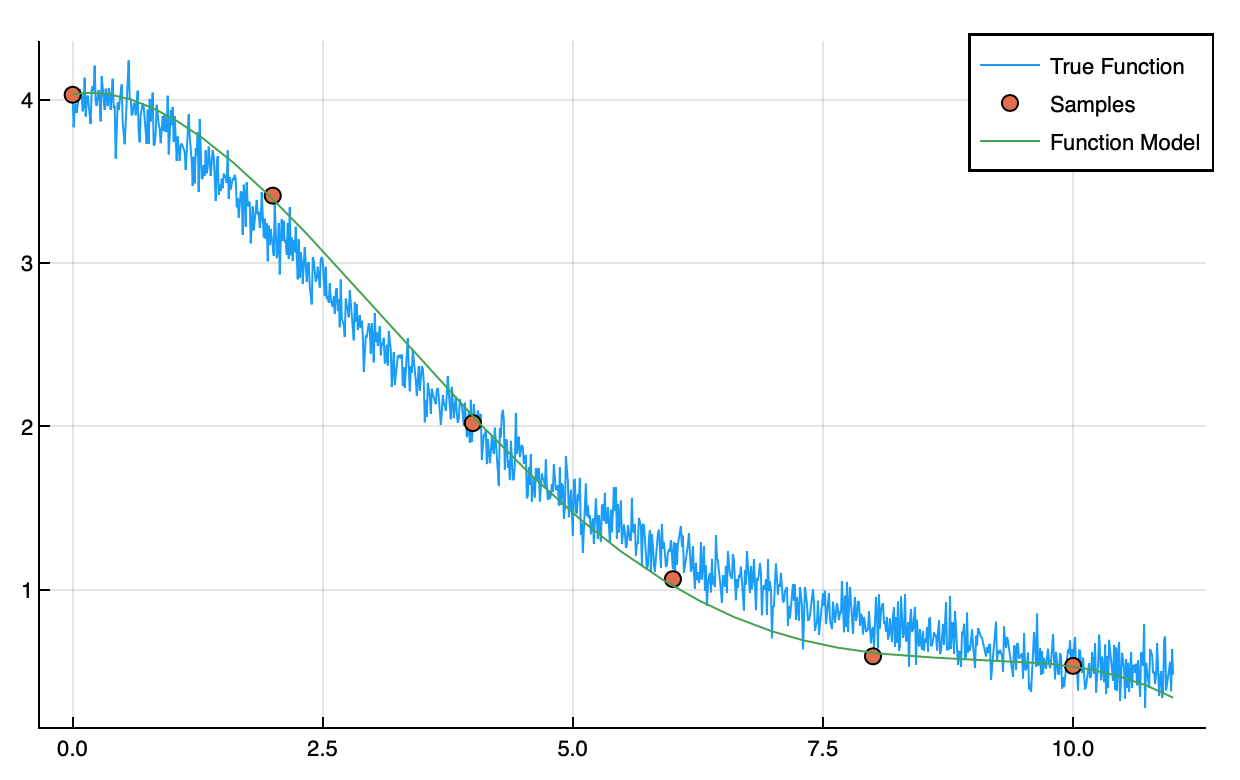
\includegraphics[scale = 0.4]{Figures/func1True}
\caption{The true function is shown by the blue line and the points are the locations of our samples. The green line shows the function created by our model to predict the true function.
\label{figFunc1True}} 
\end{figure}



\subsection{Basis Functions and Sample Size}\label{Sect:samplesAndFunctions}
\par As seen in the previous section, and in particular Equations \ref{LinAlgSubscript} and \ref{realValues}, each row of matrix $A$ and vector $\vec{y}$ represents a single sampling and each column is a unique basis function. It should be understood that as either of these two variables increases, thus increasing the length or width of $A$, so should the accuracy and precision of the model increase. In theory, there is no limit to the number of samples or basis vectors that could be used to construct a model, but in reality, there is a balance between the former variables and computational capabilities. In the example given, an increase in the number of samples or basis functions will not dramatically affect the computational power required, but becomes a greater concern for models of systems with increasing complexity. 
\par As discussed, the quantity of basis functions can make a large impact, but another important factor is quality. Though the choice of basis functions in the example above was simple, it can often be a difficult choice. Consider, for example, a Fourier basis. The equivalent of Equation \ref{LinAlgSubscript} in this basis would be

\begin{equation} \label{fourierBasis}
\begin{bmatrix}
\sin(x_1) & \sin(2x_1) \\
\sin(x_2) & \sin(2x_2) & \ldots & \ldots \\
\sin(x_3) & \sin(2x_3) \\
\vdots & & \ddots & & \\
\sin(x_n) & \ldots & & \sin(mx_n)
\end{bmatrix}
\begin{bmatrix}
b_0 \\
b_1 \\
b_2 \\
\vdots \\
b_m 
\end{bmatrix}
=
\begin{bmatrix}
f(x_1) \\ 
f(x_2) \\
f(x_3) \\ 
\vdots \\
f(x_n)
\end{bmatrix},
\end{equation}
for an $n\times m$ matrix.
\par When used in the proper circumstance, this Fourier basis can be an excellent choice for modeling a function, as in Figure \ref{2dFourier}.

\begin{figure}[h]
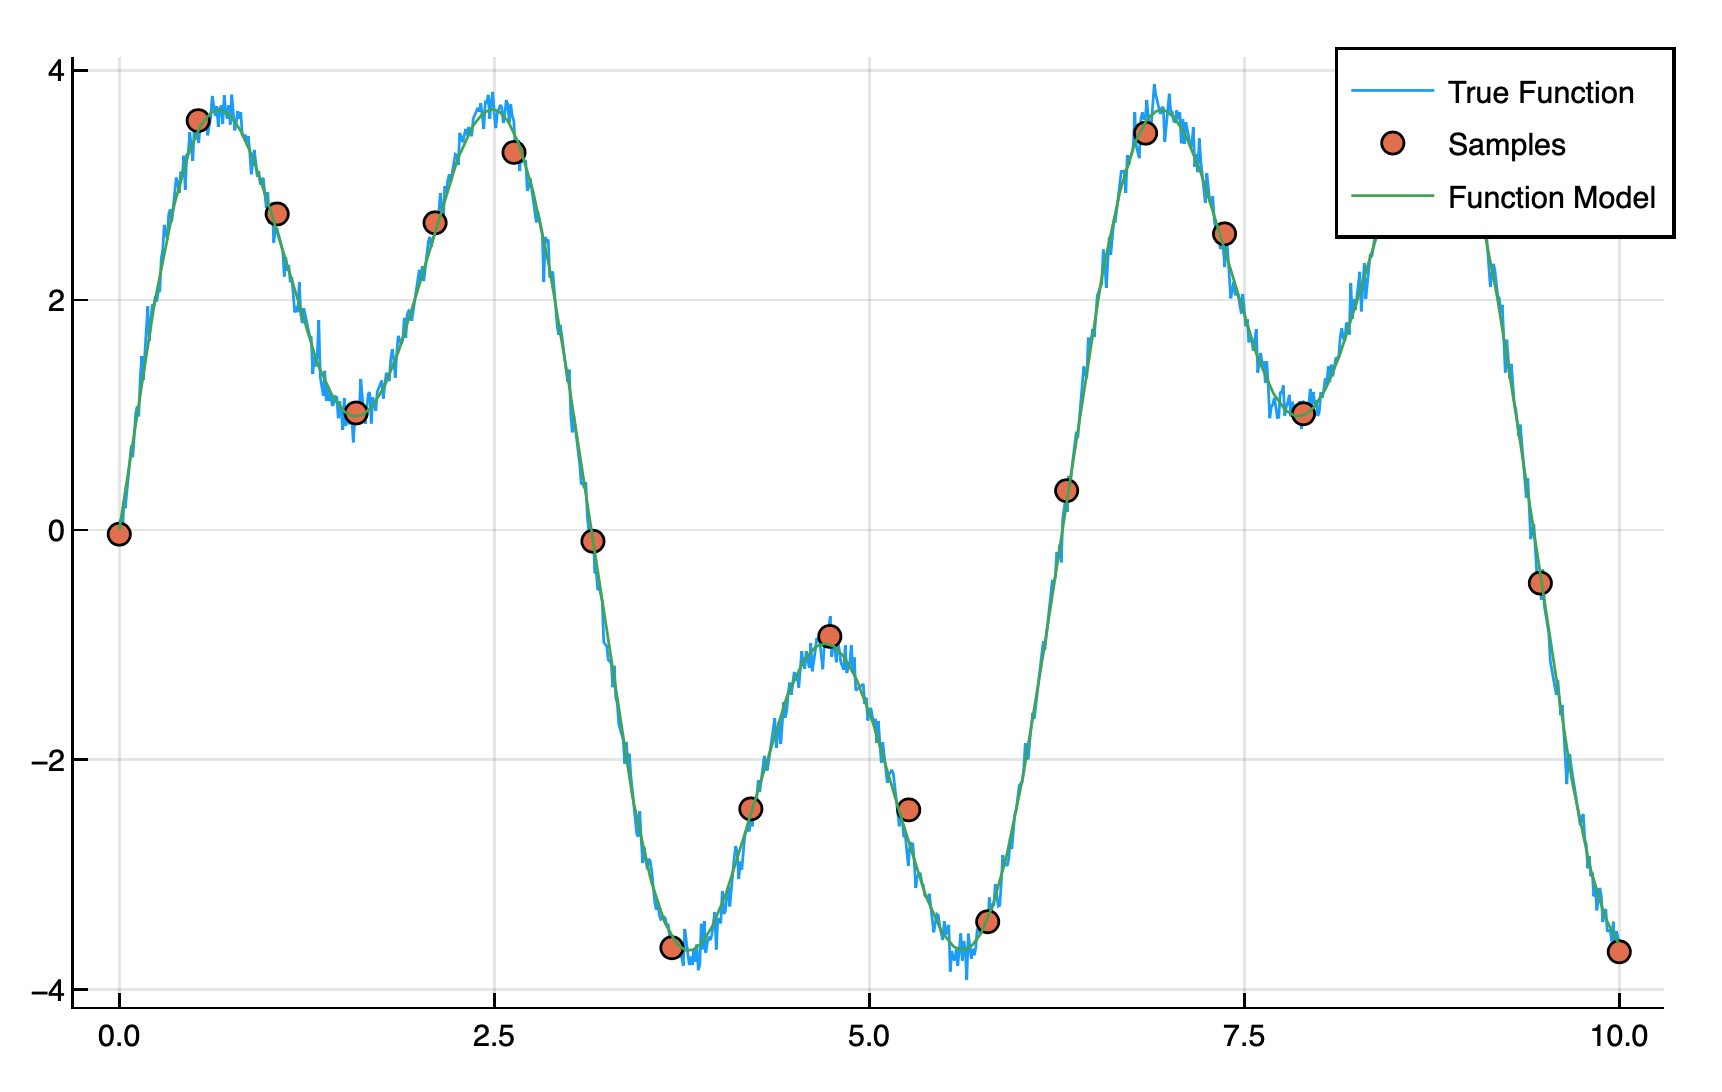
\includegraphics[scale = 0.27]{Figures/2dFourier}
\caption{The sample points shown were used to build a model of the function in green, and the true function is displayed in blue. As can be seen, a Fourier basis resulted in an excellent fit. 
\label{2dFourier}} 
\end{figure}

\par When chosing sample points, there are again two things to consider: number and breadth. As will be seen later, the number of samples can have a significant impact on the time it takes to construct a model and the accuracy of said model. The breadth of samples is similarly important. If all samples from Figure \ref{2dFourier} were taken between 0 and 1, the model produced would poorly estimate $f(2.5)$, as in \ref{poorSamps}. 

\begin{figure}[h]
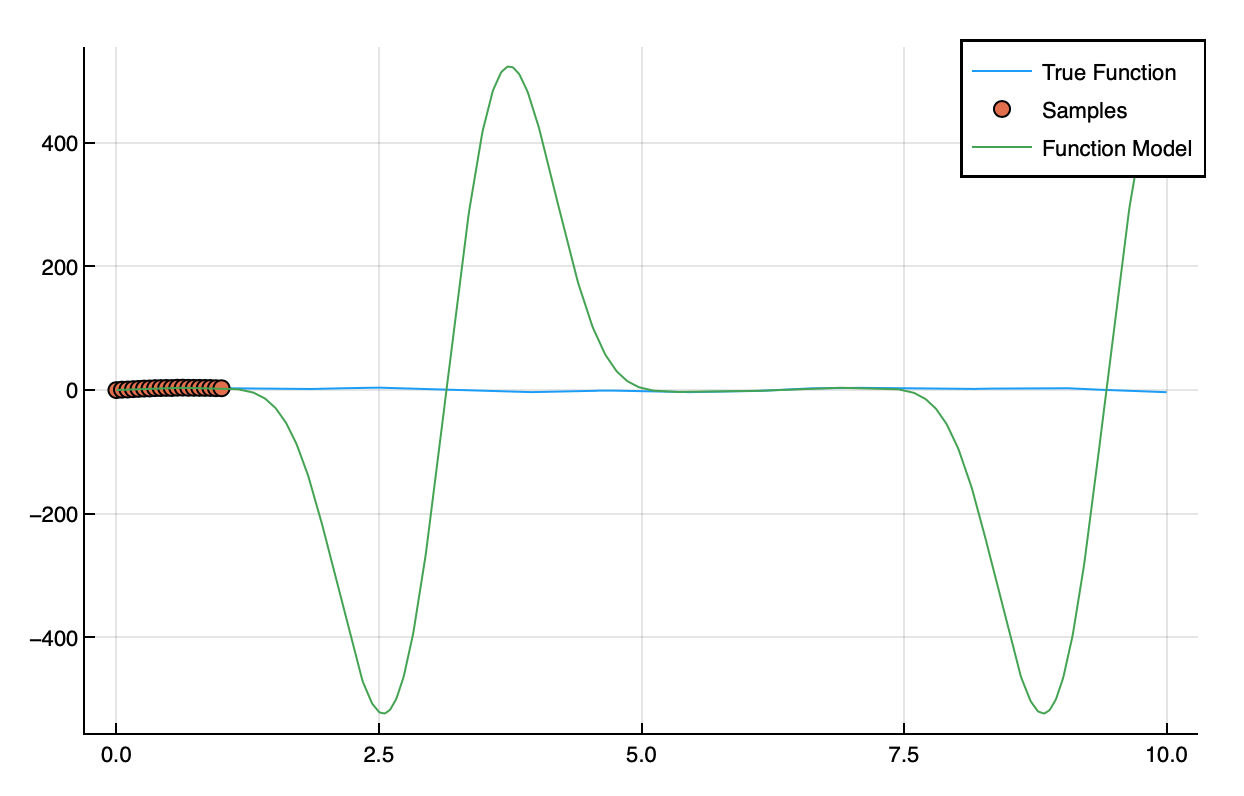
\includegraphics[scale = 0.4]{Figures/poorSamps}
\caption{A model with an insufficient breadth of samples will naturally produce a poor model. In this case, samples were only taken from the interval 0 to 1. If the model were evaluated at $x=2.5$, the fit would produce a highly inaccurate result when compared to the true function.
\label{poorSamps}} 
\end{figure}

\par By this point it should be obvious to the reader that the decision of number and breadth of sample points as well as quantity and quality of basis functions is critical to the model's performance. With well chosen basis functions but poor breadth of samples, a model's accuracy can be greatly limited, as in Figure \ref{poorSamps}. Figure \ref{3dFourier} shows the reverse situation, good number and breadth of samples, but poorly chosen basis functions. 

%\begin{figure}[h]
%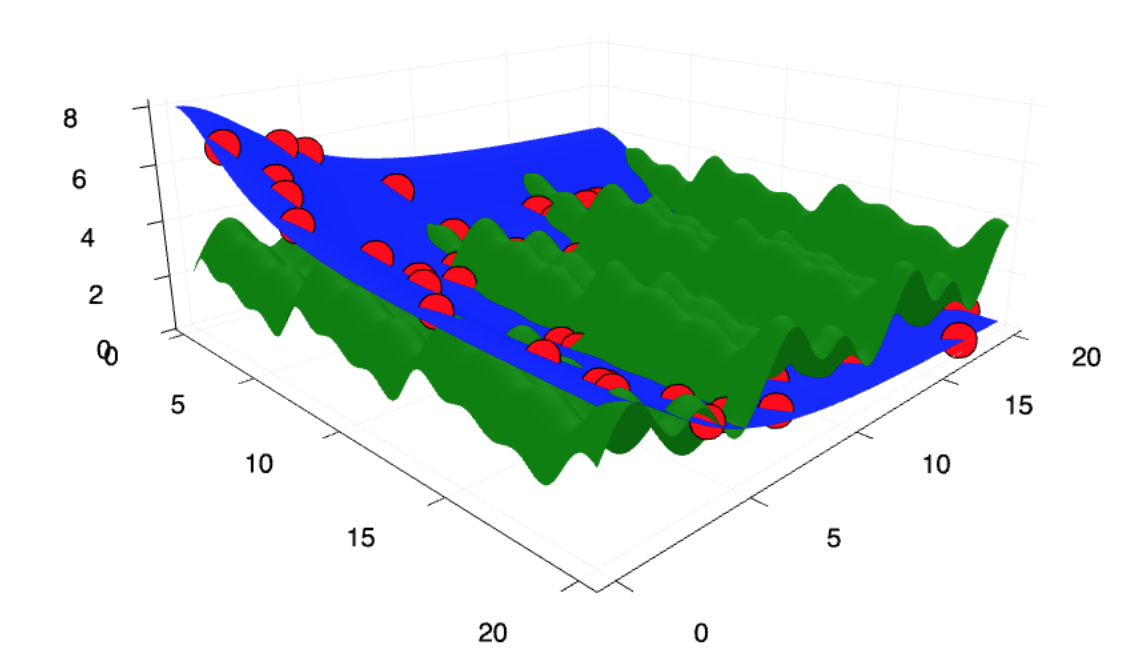
\includegraphics[scale = 0.42]{Figures/3dFourier}
%\caption{A three dimensional function in blue with a constructed model in green. The red points show the sampling of the true function. In this case, a Fourier basis is a poor choice and resulted in an inaccurate model of the true function.
%\label{3dFourier}} 
%\end{figure}

\begin{figure}
  \begin{subfigure}{0.35\textwidth}
    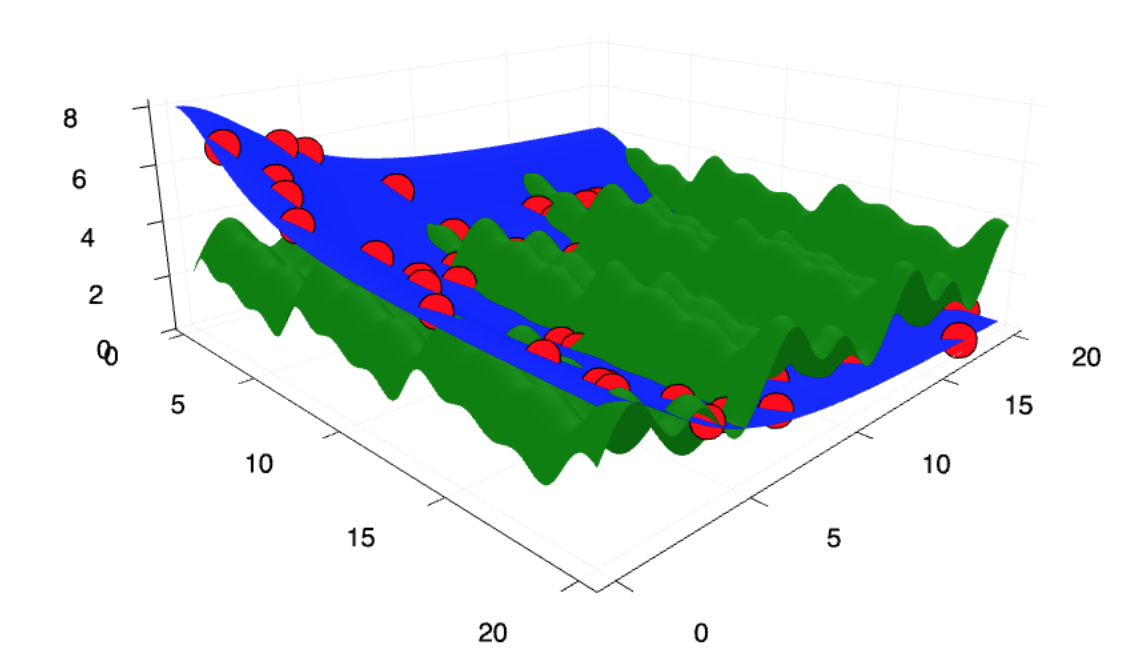
\includegraphics[width=\linewidth]{Figures/3dFourier}
    \caption{Fourier basis. $A$ is a $50\times7$ matrix.} 
    \label{3dFourier}
  \end{subfigure}%
  \\
  \begin{subfigure}{0.35\textwidth}
    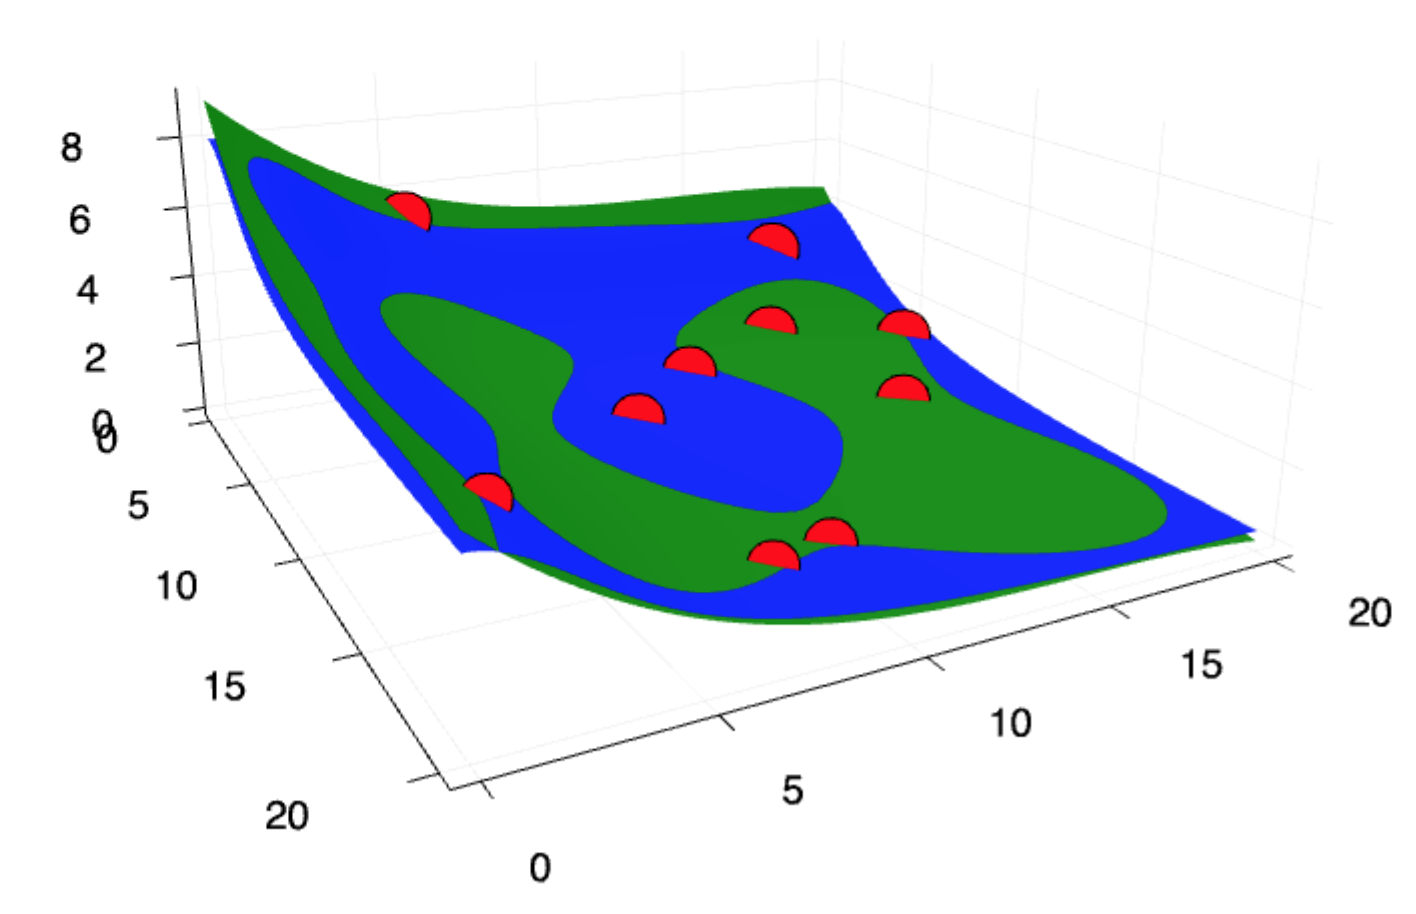
\includegraphics[width=\linewidth]{Figures/3dPower}
    \caption{Power basis. $A$ is a $10\times7$ matrix.} 
    \label{3dPower}
  \end{subfigure}%
\caption{A three dimensional function in blue with a constructed model in green. The red points show the sampling of the true function. (a) In this case, a Fourier basis is a poor choice and resulted in an inaccurate model of the true function. (b) A Power series makes a convincingly better fit even with significantly fewer sample points.} \label{3dFit}
\end{figure}


\subsection{Julia}\label{Sect:julia}
The figures provided throughout this paper were produced using the Julia programming language. Though encouraged to use Python for the majority of my formal education, Julia is a relatively new and fast growing language in terms of popularity. 
